\section{Metodología seguida}
Se define metodología \cite{metodologiaRAE}, como los métodos y pasos seguidos con el objetivo de desarrollar o fabricar algo, de manera que el resultado final sea acorde a los resultados y calidad esperados del mismo. De esta forma, es posible cumplir con los plazos de entrega del producto o servicio, a la vez que se obtiene un resultado acorde a lo establecido. 

\subsection{Procesos Unificados de Desarrollo}
En la actualidad, es posible encontrar innumerables metodologías para gestionar un proyecto de cualquier tipo. Si bien es imposible o muy difícil adecuarse por completo a una sola metodología, es posible decantarse por un conjunto reducido o incluso una sola en función del objetivo del proyecto a desarrollar. En este trabajo se ha emplear una metodología basada en \ac{PUD} \cite{libro-PUD} \cite{PUD-2}, centrada en el enfoque iterativo e incremental con el objetivo de aportar un mayor valor conforme avanza el proyecto a realizar. Como principales razones para esta elección destacan las siguientes:

\begin{itemize}
\item El proyecto se organiza de manera estructurada en iteraciones 
\item Cada iteración puede verse como un micro-proyecto, permitiendo, si es necesario, la aplicación de metodologías distintas, dando gran flexibilidad.
\item Los resultados de cada iteración sirven como base para la siguiente, aumentando progresivamente el valor del proyecto a medida que éste avanza.
\item No se necesita definir todos los requisitos al comienzo, es posible realizar ajustes en iteraciones previas sin dificultad.
\item Agiliza el desarrollo del proyecto al generar resultados a corto plazo
\end{itemize}

En la metodología PUD, el esfuerzo se divide en fases, cada una tomando unas entradas, y generando unas salidas, las cuales serán la entrada de la siguiente fase a realizar. El conjunto de todas las fases es lo que se conoce como ciclo. Así pues, un ciclo está compuesto de las siguientes fases:

\begin{enumerate}
    \item \textbf{Inicio:} Se describe del resultado esperado al fin de la iteración.
    \item \textbf{Elaboración:} Se detallan los casos de uso que a considerar durante la iteración.
    \item \textbf{Construcción:} Se modela el resultado de la iteración a partir de los casos de uso. En caso de fallo de los requisitos, se realimenta la fase hasta obtener un resultado correcto.
    \item \textbf{Transición:} Se valida el resultado generado en la iteración. En caso de fallo de los requisitos, se realimenta la fase hasta obtener un resultado correcto.
\end{enumerate}

En este trabajo este ciclo se repetirá las veces necesarias para cumplir con los objetivos planteados en el mismo.

\subsection{Iteraciones realizadas}
A modo de esquema, se presenta en \ref{tbl:cicloIteraciones} una tabla relacionando las iteraciones realizadas en este proyecto, fechas de inicio/fin, descripciones, dentro del único ciclo de PUD realizado. Para finalizar, se presenta en \ref{fig:gantt} el diagrama de Gantt equivalente.

\begin{table}[H]
    \centering
    \resizebox{15.5cm}{!} {
        \begin{tabular}{|c|c|c|c|c|}
        \hline
        \rowcolor[HTML]{C0C0C0} 
        \textbf{FASE} & \textbf{ITERACIÓN} & \textbf{DESCRIPCIÓN} & \textbf{INICIO} & \textbf{FINAL} \\ \hline
        \cellcolor[HTML]{EFEFEF}Inicio & 1 & Modelo del sistema & 31/05/2025 & 15/06/2025 \\ \hline 
        \cellcolor[HTML]{EFEFEF} & 2 & Desarrollo del diseño hardware & 10/06/2025 & 31/07/2025 \\ \cline{2-5} 
        \multirow{-2}{*}{\cellcolor[HTML]{EFEFEF}Elaboracion} & 3 & Ejecución de simulaciones funcionales & 01/08/2025 & 10/08/2025 \\ \hline
        \cellcolor[HTML]{EFEFEF} & 4 & Integración del diseño en X-HEEP & 11/08/2025 & 25/08/2025 \\ \cline{2-5} 
        \multirow{-2}{*}{\cellcolor[HTML]{EFEFEF}Construccion} & 5 & Ejecución del diseño en X-HEEP sobre FreeRTOS & 16/08/2025 & 01/09/2025 \\ \hline
        \cellcolor[HTML]{EFEFEF} & 6 & Comparativa de resultados frente a versión software & 30/08/2025 & 03/09/2025 \\ \cline{2-5} 
        \multirow{-2}{*}{\cellcolor[HTML]{EFEFEF}Transicion} & 7 & Documentación del proyecto & 01/08/2025 & 05/09/2025 \\ \hline
        \end{tabular}
    }
    \caption{Iteraciones identificadas en el proyecto}
    \label{tbl:cicloIteraciones}
\end{table}


\begin{figure}[!ht]
  \centering
    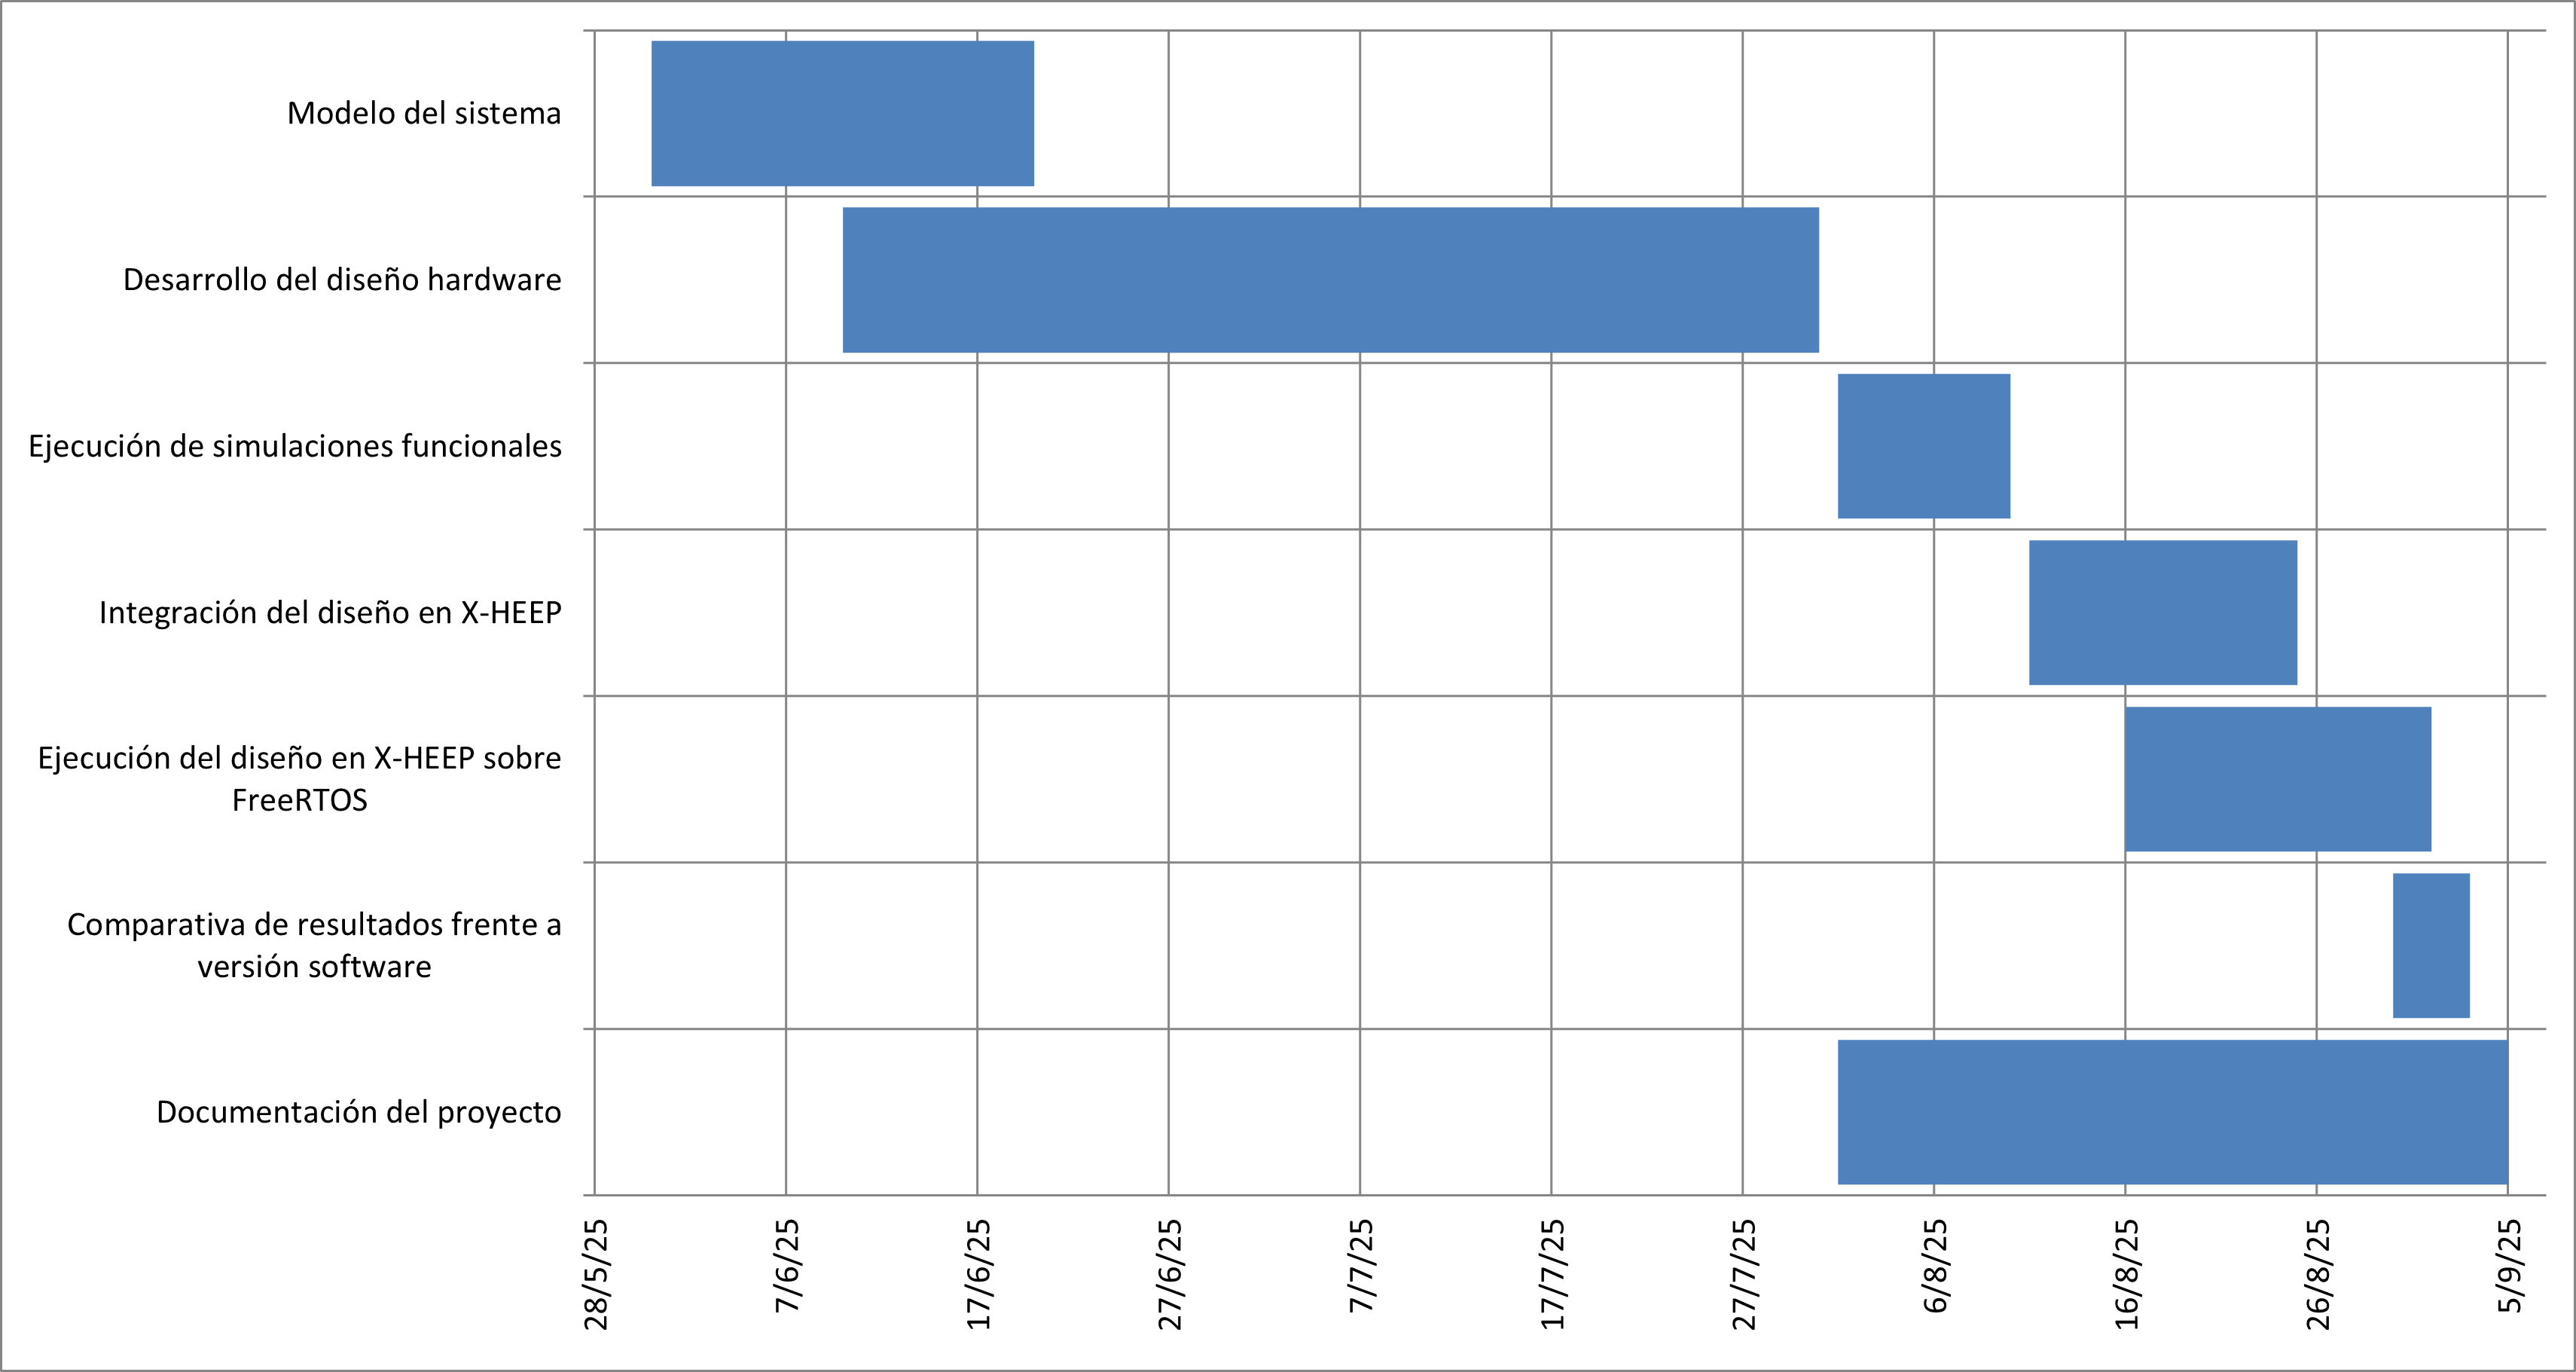
\includegraphics[width=15cm]{figures/gantt.png}
  \caption{Diagrama de Gantt}
  \label{fig:gantt}
\end{figure}


\section{Análisis de requisitos}
\label{sec:requisitos}
Los requisitos identificados en el proyecto son:

\begin{itemize}
    \item Desarrollar una aplicación en \textit{hardware}
    \item Emplear metodologías basadas en herramientas EDA
    \item Hacer uso del protocolo de comunicaciones AXI-Stream
    \item Validar la funcionalidad del diseño realizado
    \item Integración del diseño en X-HEEP
    \item Ejecutar el diseño en X-HEEP sobre FreeRTOS
    \item Comparar el rendimiento con una versión \textit{software}
\end{itemize}

El cumplimiento (completo o parcial) o incumplimiento de los requisitos tenidos en cuenta en este trabajo se valorará posteriormente, en el capítulo \ref{cap:conclusiones}.

\section{Arquitectura de la solución}

\subsection{Componentes funcionales}
En el proyecto se ha llevado a cabo una solución basada en diagramas de bloques (\textit{block design}) dde carácter modular, donde cada bloque presenta una funcionalidad específica, y su agrupación permite realizar funciones de major complejidad. Concretamente, se han realizado los siguientes bloques:

\begin{enumerate}
    \item Una cola de entrada de datos, que permite la entrada de enteros de 32 bits, así como una señal de comienzo (\emph{start}) que arranca el diseño globalmente.
    \item Una versión acelerada por \textit{hardware} del algoritmo de reverso de bits (\emph{bit reversal}) realizada con el programa Vitis HLS, e importado a Vivado
    \item Una cola de salida de datos, que permite obtener el resultado final tras aplicar el reverso, así como una señal de terminado (\emph{done}) para saber en qué momento se tienen resultados.
\end{enumerate}

Estos elementos se han integrado en un Block Design en Vivado, que es el que instancia a todos ellos, tal y como puede verse en \ref{fig:proyectoVivado}.

\subsection{Interfaces utilizadas}
Para la interconexión de los módulos de las colas con el acelerador en cuestión, se ha hecho uso del conocido protocolo \ac{AXI} Stream, donde se ha realizado una implementación reducida, teniendo en cuenta, por simplicidad, el menor número de señales posible: \emph{datos, ready, valid, last}. En la figura \ref{fig:proyectoVivado} puede apreciarse estas conexiones citadas.

Además de AXI, es necesario utilizar otro protocolo para poder integrar el diseño en X-HEEP: \ac{OBI}, protocolo libre de licencias y utilizado en los SoCs RISC-V, RI5CY y LowRISC-Ibex \textit{cores} \cite{infoOBI}, como el CV32E40P. Este protocolo es similar a AXI, y se basa igualmente en un esquema \emph{request-response}.

\subsection{Componentes técnicos}
Si bien las herramientas principales, empleadas para el diseño de la solución, ya han sido detalladas:

\begin{itemize}
    \item \textbf{Vivado Design Suite}: en \ref{st:vivado}
    \item \textbf{X-HEEP}: en \ref{st:xheep}
    \item \textbf{FreeRTOS}: en \ref{st:freertos}
    \item \textbf{EdaPlayground}: en \ref{st:edaplayground}
\end{itemize}

Se ddebe, como mínimo, presentar una serie de herramientas extra, clave para el despliegue técnico del proyecto, destacando:

\begin{itemize}
    \item \textbf{Vitis HLS}: \cite{vitisHLSInfo} herramienta que convierte un algoritmo en C a código HDL como Verilog, clave para poder integrarlo con otros módulos en \textit{hardware}. 
    \item \textbf{Make}\cite{makeInfo}: herramienta para compilar la plataforma de X-HEEP
    \item \textbf{RISC-V GCC-Toolchain}\cite{gccRISCVInfo}: para compilar programas RISC-V con \ac{GCC}
    \item \textbf{Visual Studio Code}\cite{vscodeInfo}: como el \ac{IDE} empleado para el desarrollo técnico del proyecto
\end{itemize}

Hay que presentar también herramientas utilizadas en la gestión del proyecto a nivel global:

\begin{itemize}
    \item \textbf{\href{https://git-scm.com/downloads}{Git}}: es un \ac{DVCS}, sistema de control de versiones distribuido, que permite mantener un historial del código desarrollado en cada momento, pudiendo volver atrás si es necesario. En Git, un proyecto está compuesto por un \emph{repositorio}, o un conjunto de éstos.
    \item \textbf{\href{https://github.com/}{GitHub}}: plataforma donde los usuarios pueden alojar repositorios Git y registrar los cambios realizados. Para este trabajo, se ha creado un repositorio, al cual puede accederse \href{https://github.com/fluctlights/perte_tfm} {en este enlace}
    \item \textbf{\href{https://clickup.com/}{ClickUp}}: herramienta web de gestión de proyectos. Permite conocer el estado en todo momento y a planificar diagramas de Gantt cómodamente, entre otros.
\end{itemize}

Y finalmente, las herramientas utilizadas en la redacción de este proyecto son:

\begin{itemize}
    \item \textbf{\href{https://www.latex-project.org/get/}{\LaTeX}}: sistema de procesamiento de documentos basado en TeX, muy popular en el ámbito académico, principalmente por la alta calidad de los documentos finales, lo que facilita la lectura.
    \item \textbf{\href{https://marketplace.visualstudio.com/items?itemName=James-Yu.latex-workshop}{Latex Workshop}}: extensión para Visual Studio Code que proporciona soporte a características y compilación para documentos \LaTeX.
    \item \textbf{\href{https://www.drawio.com/}{Drawio}}: editor web que sirve, entre otros, para haber realizado los diagramas presentes en el trabajo, con gran facilidad y flexibilidad de uso.
    \item \textbf{\href{https://www.tablesgenerator.com/}{Tables Generator}}: editor web empleado para realizar las tablas presentes en el trabajo.
    \item \textbf{\href{https://www.microsoft.com/es-es/microsoft-365/excel}{\ac{MS} Excel}}: gestor de hojas de cálculo polivalente, empleado en este trabajo para ordenar datos y generar las tablas comparativas de rendimiento entre diseño desarrollado y versión puramente software.
\end{itemize}

\subsection{Implementación e infraestructura}
La implementación del proyecto se ha realizado en tres fases bien diferenciadas:

\begin{enumerate}
    \item \textbf{Desarrollo del algoritmo \textit{bit reversal}}: mediante la herramienta Vitis HLS, se ha generado el código RTL necesario para realizar la implementación en \textit{hardware}.
    \item \textbf{Creación del diseño basado en \emph{block design}}: mediante Vivado Design Suite se ha realizado y simulado con \textit{testbenchs} un diseño basado en colas que utiliza AXI-Stream para comunicarse con el acelerador desarrollado.
    \item \textbf{Integración del diseño en X-HEEP sobre FreeRTOS}: se hace uso de un \textit{fork} de X-HEEP llamado GR-HEEP \cite{grheepInfo} para ejecutar software en C con las librerías de FreeRTOS y haciendo uso del diseño creado. Será precisamente esta integración la intraestructura final sobre la que se sostenga el trabajo.
\end{enumerate}
